\subsection{Decoherence in the Combiner Ring \textbf{Tobias}}

One of the targets for CTF3 is to demonstrate a combined beam with emittance
below \unit[150]{$\pi\mu$m} for both planes \cite{roberto_telavi_linac}.
There are several factors that can increase the emittance in the combiner
ring, such as uncontrolled dispersion, unmatched lattice and miss-steering
at injection. A study was launched in 2012 to understand where the observed
increase was originating from. It was found that injecting onto the closed
orbit of the combiner ring was of key importance to minimize the emittance
growth. The emittance increase is caused by the large energy spread of the
beam in combination with high chromaticity in the combiner ring. 
The effect of decoherence is shown in figure~\ref{fig:decoherence} and described in
section~\ref{sec:aboutdechorense}. In figure~\ref{fig:emittance_growth} the
standard deviation around the closed orbit for a short pulse circulating 4
turns is plotted against the horizontal emittance. I varied the magnitude of
the oscillations around the closed orbit by changing corrector magnets
before the injection. The standard deviation is measured using 5 BPMs, the
quoted standard deviation is the mean of these value. It was repeated with a
beam combined 4 times. As seen in figure~\ref{fig:emittance_growth} the
emittance for this beam is larger than for the uncombined beam. 
The reason is that the different turns have slightly different orbits and 
hence they are together occupying a larger part of the transverse space. 
The measurements of the uncombined beam show good agreement with simulations
\cite{clic_workshop_cern_emittance}. 

\begin{figure}[!h]
\begin{center}
%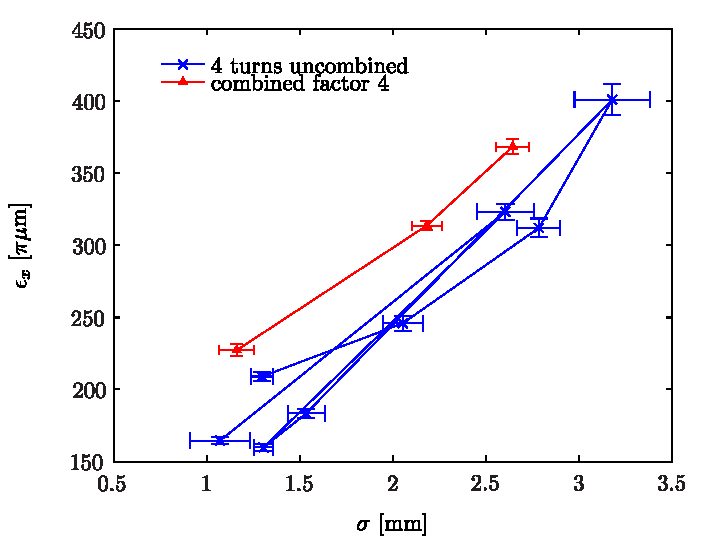
\includegraphics[height=8.4cm,natwidth=341,natheight=262]{emittance_growth.pdf}
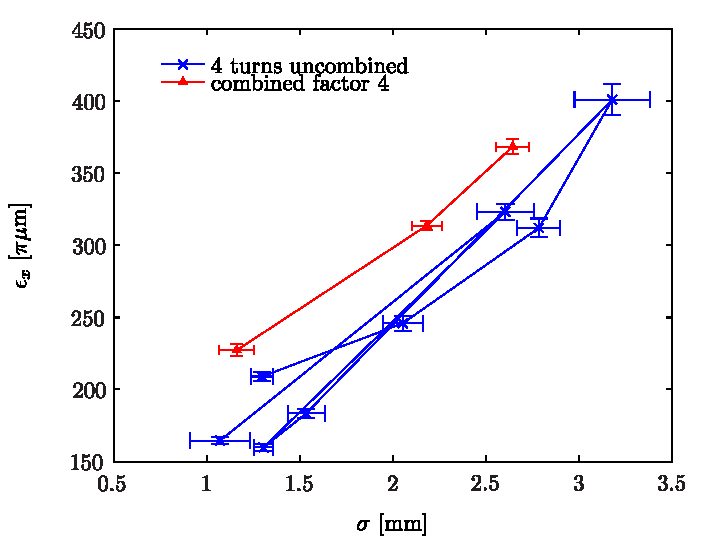
\includegraphics[height=8.4cm]{emittance_growth.pdf}
\end{center}
\caption{The horizontal emittance as a function of amplitude of the oscillations around the closed orbit. }
\label{fig:emittance_growth}
\end{figure} 

After a careful setup of the injection and extraction to the combiner ring 
a Drive Beam emittance of \unit[150]{$\pi \mu$m} was achieved for a factor 4 combined beam. 
The result is presented in Paper~\cite{ipac_ctf3_2013} together with a summary of recent achievements in CTF3. 
\todo{There should be another one with roughly the same values I think from later..}
